\documentclass[a4j]{jarticle}
    \usepackage[dvipdfmx]{graphicx}
    \usepackage[ top=25truemm,bottom=37truemm,left=25truemm,right=25truemm]
    {geometry}
    \usepackage{ascmac}
    \usepackage{array}
    \usepackage{here}
    \usepackage{url}
    \usepackage{listings, jlisting}
    \usepackage{tikz}
    \usetikzlibrary{intersections,calc,arrows}
    \renewcommand{\lstlistingname}{リスト}
\lstset{language=c,
  basicstyle=\ttfamily\scriptsize,
  commentstyle=\textit,
  classoffset=1,
  keywordstyle=\bfseries,
  frame=tRBl,
  framesep=5pt,
  showstringspaces=false,
  numbers=left,
  stepnumber=1,
  numberstyle=\tiny,
  tabsize=4
}

\makeatletter
\def\@thesis{シミュレーション レポート}
\def\id#1{\def\@id{#1}}
\def\department#1{\def\@department{#1}}

\def\@maketitle{
\begin{center}
{\huge \@thesis \par} %修士論文と記載される部分
\vspace{10mm}
{\LARGE\bf \@title \par}% 論文のタイトル部分
\vspace{10mm}
{\Large \@date\par}	% 提出年月日部分
\vspace{20mm}
{\Large \@department \par}	% 所属部分
{\Large 学籍番号 \@id \par}	% 学籍番号部分
\vspace{10mm}
{\Large 氏名 \@author}% 氏名 
\end{center}
\par\vskip 1.5em
}

\title{第1回~第5回}
\date{実験日1 2020年7月15日 1~2コマ目}
\department{組番号 408}
\id{17406}
\author{金澤雄大}

    \begin{document}
    \maketitle
    \thispagestyle{empty}
    \clearpage
    \addtocounter{page}{-1}
    \section{目的}
    シミュレーションの授業の理解度を測るために,次の5つのアルゴリズムについてプログラムを作成することを目的とする.
    また作成したプログラムの誤差や収束の様子を比較し,考察することを目的とする.
  \begin{enumerate}
  \item 台形公式
  \item シンプソンの公式
  \item オイラー法
  \item ホイン法
  \end{enumerate}
  
    \section{実験環境}
      実験環境を表\ref{env}に示す.gccはWIndows上で動作するWSL(Windows Subsystem for Linux)で動作するものを用いる.
      \begin{table}[H]
        \caption{実験環境}
      \label{env}
      \begin{center}
          \begin{tabular}{c|l}\hline
            CPU & AMD Ryzen 5 3600 6-Core Processor \\ 
            メモリ & 16.0GB DDR4 \\
            OS & Microsoft Windows 10 Home \\
            gcc & (Ubuntu 9.3.0-17ubuntu1~20.04) 9.3.0 \\
            Make & GNU Make 4.2.1 \\ \hline
          \end{tabular}
      \end{center}
      \end{table}

    \section{課題1}
    本章では課題1における課題内容,プログラムの説明,実験結果,考察の4つについて述べる.
    \subsection{課題内容}
    課題1の課題内容は台形公式を用いて式(\ref{kadai1siki})を数値積分するものである.式(\ref{kadai1siki})の解析解は$\frac{1}{2} \log_{e} 3$である.
    分割数を1,2,4というように$\frac{1}{2}$ずつ細かくしたときの,台形公式で求めた積分値と解析解の関係について考察する.
    \begin{equation}
  \int_0^\frac{\pi}{6} \frac{dx}{\cos x}
      \label{kadai1siki}
    \end{equation}

    \subsection{プログラムの説明}
    本節では課題1で作成したプログラムおいて,次に示す4つの関数の役割および機能について説明する.なお数学における「関数」とプログラミング
    における「関数」の意味が混在することを防ぐため,数学における関数を「数学関数」,プログラミングにおける関数を「関数」と表記する.
    \begin{enumerate}
      \item func関数
      \item Trapezoidal関数
      \item TrapezoidalRule関数
      \item main関数
      \end{enumerate}
    
    \subsubsection{func関数}
    func関数は数値計算を行う数学関数を定義する関数である.表\ref{func1table}にfunc関数の機能,引数,返り値の3つを示す.
    func関数は数学関数を定義する関数であるから,引数$x$(double型)について返り値$f(x)$を返す設計になっている.
      \begin{table}[H]
      \caption{func関数の機能,引数,返り値}
      \label{func1table}
      \begin{center}
          \begin{tabular}{c|l}\hline
        機能 & 数学関数を定義する\\
        引数 & double x \\
        返り値 & double型 \\ \hline
          \end{tabular}
      \end{center}
      \end{table}

    リスト\ref{func1}にfunc関数のソースコードを示す.func関数は引数xについて積分を行う数学関数$f(x) = \frac{1}{\cos x}$の値を
    返す.なおcos関数を扱うためにはmath.hのincludeが必要である.
    \begin{lstlisting}[basicstyle=\ttfamily\footnotesize, frame=single,label=func1,caption=func関数]
double func(double x){
    return 1/cos(x);
} 
    \end{lstlisting}

    \subsubsection{Trapezoidal関数}
    Trapezoidal関数は数学関数$f(x)$において,与えられた2点$a$,$b$における台形公式による数値積分を行う関数である.
    2点$a$,$b$における$f(x)$の値は$f(a)$,$f(b)$であるから,$a$から$b$までの$f(x)$の積分は台形公式より式(\ref{simpleTrapezaidal})のように
    近似できる.
    \begin{equation}
      \int_a^b f(x) dx \simeq \frac{b-a}{2}(f(a)+f(b))
          \label{simpleTrapezaidal}
        \end{equation}

    表\ref{Trapezoidaltable}にTrapezoidal関数の機能,引数,返り値の3つを示す.Trapezoidal関数は2点$a$,$b$における台形公式による数値積分
    を行う関数であるから,2点$a$,$b$を引数,数値積分の結果の返り値とする設計になっている.
    \begin{figure}[H]
      \centering
    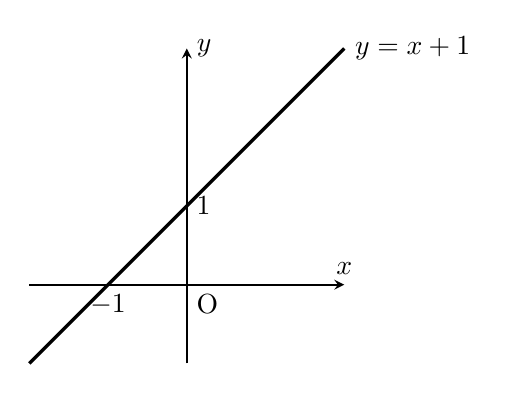
\begin{tikzpicture}
 \draw[->,>=stealth,semithick] (-2,0)--(2,0)node[above]{$x$}; %x軸
 \draw[->,>=stealth,semithick] (0,-1)--(0,3)node[right]{$y$}; %y軸
 \draw (0,0)node[below right]{O}; %原点
 \draw (-1,0)node[below]{$-1$}; %点(-1,0)
 \draw (0,1)node[right]{$1$}; %点(0,1)
 \draw[very thick,domain=-2:2] plot(\x,\x+1)node[right]{$y=x+1$};
\end{tikzpicture}
\caption{M1} \label{fig:M1}
\end{figure}

    \begin{table}[H]
      \caption{Trapezoidal関数の機能,引数,返り値}
      \label{Trapezoidaltable}
      \begin{center}
          \begin{tabular}{c|l}\hline
        機能 & 2点$a$,$b$における台形公式による数値積分を返す.\\
        引数 & double a,double b\\
        返り値 & double型 \\ \hline
          \end{tabular}
      \end{center}
      \end{table}

      リスト\ref{Trapezoidal}にTrapezoidal関数のソースコードを示す.Trapezoidal関数は引数$a$,$b$について
      式(\ref{simpleTrapezaidal})の計算結果を返す.
      \begin{lstlisting}[basicstyle=\ttfamily\footnotesize, frame=single,label=Trapezoidal,caption=Trapezoidal関数]
double Trapezoidal(double a,double b){
    return (b-a)*(func(a)+func(b))/2;
}
            \end{lstlisting}

    \subsubsection{TrapezoidalRule関数}
    TrapezoidalRule関数は区間[$a$,$b$]を$n$個に分割して,分割した区間のそれぞれに台形公式を適用する関数である.

    \subsubsection{main関数}

    \subsection{実行結果}
    \subsection{考察}

    \section{課題2}
    本章では課題2における課題内容,プログラムの説明,実験結果,考察の4つについて述べる.
    \subsection{課題内容}
    \subsection{プログラムの説明}
    \subsection{実行結果}
    \subsection{考察}

    \section{課題3}
    本章では課題3における課題内容,プログラムの説明,実験結果,考察の4つについて述べる.
    \subsection{課題内容}
    \subsection{プログラムの説明}
    \subsection{実行結果}
    \subsection{考察}

    \section{課題4}
    本章では課題4における課題内容,プログラムの説明,実験結果,考察の4つについて述べる.
    \subsection{課題内容}
    \subsection{プログラムの説明}
    \subsection{実行結果}
    \subsection{考察}

    \section{課題5}
    本章では課題5における課題内容,プログラムの説明,実験結果,考察の4つについて述べる.
    \subsection{課題内容}
    \subsection{プログラムの説明}
    \subsection{実行結果}
    \subsection{考察}

        \begin{thebibliography}{9}
          \bibitem{NNCT}  国立高専機構長野高専,閲覧日2020年8月7日
          \end{thebibliography}

\end{document}

